\documentclass{beamer}
\usepackage[brazil]{babel}
\usepackage[utf8]{inputenc}
\usepackage{times}
\usepackage[T1]{fontenc}
%\usepackage{subfigure}
%\usepackage{wrapfig}
\usepackage{float}
\usepackage{ctable}
\usepackage{colortbl}

\usepackage{pgfpages}

\mode<presentation>
{
  \usetheme{Singapore}
  \usecolortheme{rose}
  %\usefonttheme[onlylarge]{structurebold}
  %\setbeamerfont*{frametitle}{size=\normalsize,series=\bfseries}
  % or ...
  \setbeamercovered{transparent}
  % or whatever (possibly just delete it)
  \setbeamertemplate{navigation symbols}{}
  %\logo{\includegraphics[width=1.2 cm]{figuras/logo_ufes}}
  %\setbeamertemplate{footline}{%
  %\leavevmode%
  %\hbox{%
  %\begin{beamercolorbox}[wd=.5\paperwidth,ht=2.25ex,dp=1ex,right]{author in
  %    head/foot}%
  %    \usebeamerfont{author in head/foot}\insertshortauthor \hspace{.5cm}
  %    (\insertshortinstitute) \hspace{.5cm}
  %\end{beamercolorbox}%

  %\begin{beamercolorbox}[wd=.5\paperwidth,ht=2.25ex,dp=1ex,left]{title in
  %    head/foot}%
  %    \usebeamerfont{title in head/foot} \hspace{.5cm}\insertshorttitle
  %\end{beamercolorbox}}%
  %\vskip0pt%
  %}
}

% Define o tema da apresentacao (soh fica guardado nas informacoes do pdf)
\subject{Detecção de drift em sensores}
% Delete this, if you do not want the table of contents to pop up at
% the beginning of each subsection:
% \AtBeginSubsection[]
% {
%   \begin{frame}<beamer>{Sumário}
%     \tableofcontents[currentsection,currentsubsection]
%   \end{frame}
% }
% \AtBeginSection[]
% {
%   \begin{frame}<beamer>{Sumário}
%     \tableofcontents[currentsection]
%   \end{frame}
% }
%\setbeameroption{show notes}
\setbeameroption{show notes on second screen=right}
%============================================================================================

\title
[Algoritmos para a Detecção de \textit{Drifting} em Sensores de Poços de Petróleo]
{Algoritmos para a Detecção de \textit{Drifting} em Sensores de Poços de Petróleo}

\author[Boechat A.A.]
{ 
    André Ambrósio Boechat
}
\institute[UFSC]{Departamento de Automação e Sistemas\\Universidade Federal de Santa
Catarina}

%Programa de Pós-Graduação em Eng. de Automação e Sistemas\\Universidade Federal
%de Santa Catarina
%}

% Se comentar a linha abaixo, ira aparecer a data quando foi compilada a apresentacao
\date{Florianópolis, Agosto de 2012}

\setbeamercolor{postit}{fg=black,bg=block body.fg!75!black!10!bg}
% =========================================================================================
\begin{document}

\begin{frame}
    \titlepage
\end{frame}


\begin{frame}{Sumário}
    \tableofcontents[]
\end{frame}

\section{Introdução}
\subsection{}

\begin{frame}{Sensores na Indústria Petrolífera}
    \begin{itemize}
        \item Desempenham importantes papéis
            \begin{itemize}
                \item ações de controle
                \item otimização da produção
                \item monitoramento do poço
                \item monitoramento do desempenho de equipamentos
                \item tomada de decisões
            \end{itemize}
        \item Crescimento do número de sensores
        \item Localizados em pontos críticos
            \begin{itemize}
                \item difícil acesso
                \item ambientes inóspitos
            \end{itemize}
    \end{itemize}

    \begin{block}{Problema}
        As informações fornecidas pelos sensores são confiáveis?
    \end{block}

    \note{
    \begin{itemize}
        \item monitoramento do poço: mudanças nas características
        \item crescimento do número de sensores: queda dos preços
        \item ambientes inóspitos, degradantes: alta temperatura, pressão, etc.
    \end{itemize}
    }
\end{frame}

\begin{frame}{\textit{Drift} em Sensores}
    Desvio lento e continuo das medições ao longo do tempo

    \begin{itemize}
        \item Um dos problemas mais comuns em sensores
        \item Difícil detecção manual
            \begin{itemize}
                \item comparação com sinais de outros sensores
                \item detectável quando os desvios são grosseiros
            \end{itemize}
    \end{itemize}

    \begin{beamercolorbox}[sep=5pt]{postit}
        ``Leituras realizadas por um sensor instável ou com desvios excessivos
        normalmente são mais problemáticos a um operador que a falha completa do
        sensor.''\\ \footnotesize(Joseph Eck et al., 1999)
    \end{beamercolorbox}

    \begin{figure}[!htb]
        \centering
        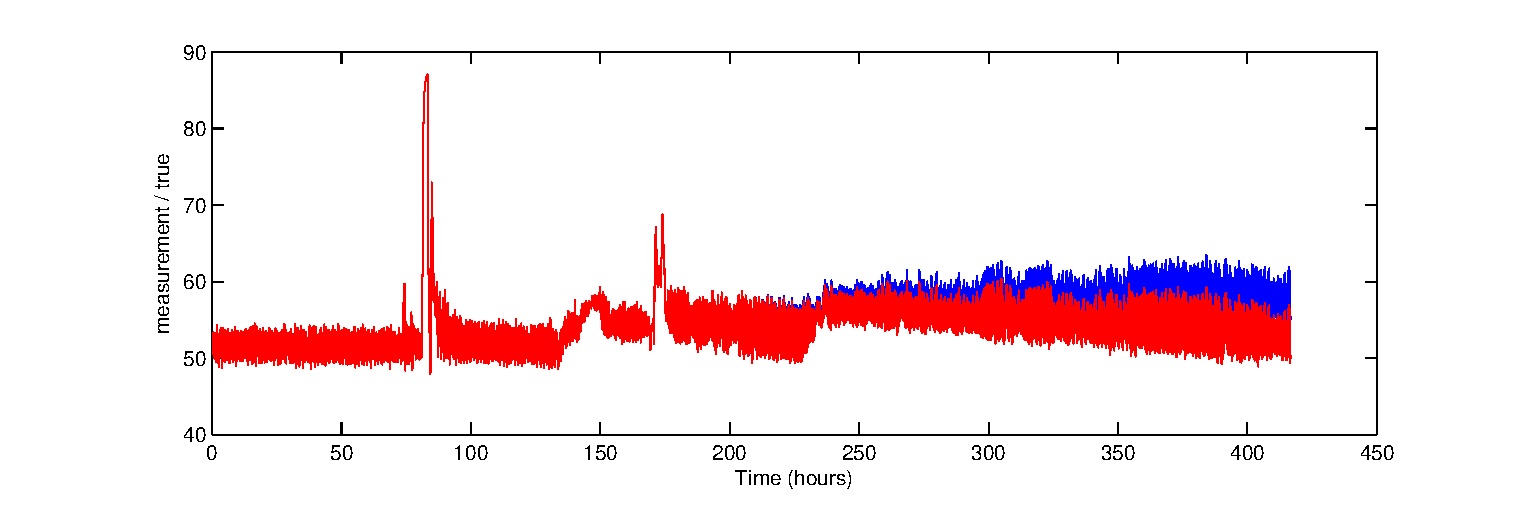
\includegraphics[trim=0pt 0pt 0cm 15pt,clip=true,width=\textwidth]{figuras/drift.eps}
    \end{figure}

    \note{
    Um dos principais problemas que ocorrem com sensores e é o foco da dissertação.

    \begin{itemize}
        \item Dificuldade de detecção manual: depende da comparação com os sinais de
            outros sensores, das ações dos operadores, além de ser perceptível apenas
            quando os desvios são grosseiros.
        \item Frase sobre falha de sensor: tomar decisões baseadas em falsas informações
            pode ser mais perigoso que decisões baseadas na falta da informação.
    \end{itemize}
    }
\end{frame}

\begin{frame}{Avaliação do Desempenho de Sensores}
    \begin{block}{Abordagem tradicional}
        \begin{itemize}
            \item calibração manual periódica
                \begin{itemize}
                    \item não se conhece a real necessidade
                    \item instrumentos são retirados de operação
                \end{itemize}
        \end{itemize}
    \end{block}

    \begin{block}{Manutenção baseada na condição (CBM)}
        \begin{itemize}
            \item monitora-se a \alert{condição} de funcionamento
            \item calibrações físicas apenas quando realmente \alert{necessário}
            \item tendem a ser menos invasivas e mais eficazes
                \vspace{6pt}
            \item redundância por \textit{hardware}
            \item redundância \alert{analítica}
                \begin{itemize}
                    \item equações fenomenológicas
                    \item modelos empíricos baseados em \alert{histórico}
                \end{itemize}
        \end{itemize}
        
    \end{block}

    \note{
    \begin{itemize}
        \item necessidade da calibração periódica: desperdício de tempo, dinheiro,
            mão-de-obra ou usa-se de forma descalibrada sem saber, mesmo que por um
            determinado período de tempo

        \item calibrações físicas no CBM: leituras podem ser ajustadas via software ou
            corrige-se as leituras conhecendo-se os erros

        \item CBM menos invasivas e mais eficazes: pelos dois motivos citados
            anteriormente sobre a calibração manual
    \end{itemize}}
    
\end{frame}

\begin{frame}{Abordagem por Modelos Baseados em Histórico}
    
    \begin{figure}[!htb]
        \centering\hspace*{-20pt}
        \includegraphics[width=1.1\textwidth]{figuras/data_driven_fdd.eps}
    \end{figure}

\end{frame}

\section{Estrutura de Sistemas de Manutenção CBM}
\subsection{}

\begin{frame}{Estrutura de Sistemas de Manutenção CBM}
    
\end{frame}

% \section{Monitoring Systems}
% \subsection{}
% 
% \begin{frame}{Sensor Drift Detection/Correction (state of art)}
%     \begin{columns}[T]
%         \column{.35\textwidth}
%         \begin{figure}
%             \centering
%             \includegraphics[height=.8\textheight]{figures/sys_arch_aakr.eps}
%         \end{figure}
%         %%
%         \column{.55\textwidth}
%         \begin{itemize}
% 
%             \item A auto-associative empirical model predicts the ``corrected'' readings
%                 of a group of correlated sensors
%                 \begin{itemize}
%                     \item kernel regression
%                     \item using historical of fault free observations
%                 \end{itemize}
%             \item The residual is analysed by statistical algorithms
%         \end{itemize}
%         
%     \end{columns}
% \end{frame}
% 
% \begin{frame}{Auto-associative Kernel Regression}
%     \begin{itemize}
%         \item \alert{Non-parametric} model
%         \item \alert{Auto-associative} arquitecture: the outputs emulate the inputs
%         \item \alert{Lazy} learning: there is not a real training procedure
%     \end{itemize}
% 
%     \centering
%     $
%     \hat{\mathbf{x}} = \frac{\sum\limits_{i=1}^n K(\mathbf{X}_i - \mathbf{x}) \;
%     \mathbf{X}_i}{\sum\limits_{i=1}^n K(\mathbf{X}_i - \mathbf{x})} 
%     $
% 
%     \begin{figure}[!htb]
%         \centering
%         \includegraphics[width=.7\textwidth]{figures/aakr_prediction.eps}
%     \end{figure}
% \end{frame}
% 
% \begin{frame}{Residual Analisys}
%     \begin{itemize}
%         \item Hypotesis:
%             \begin{itemize}
%                 \item $H_0$: \alert{normal} mode, zero mean and variance related to the sensor's
%                     noise
%                 \item $H_1$: \alert{degraded} mode, some statiscally abnormal change
%             \end{itemize}
%         \item \alert{Sequential Probability Ratio Test} (SPRT) to test the hypothesis
%     \end{itemize}
%     $$\Lambda^i = \ln \frac{P(d^i | H_1)}{P(d^i | H_0)}$$
%     $$S^i = S^{i-1} + \Lambda^i$$
%     \begin{itemize}
%         \item $A < S^i < B$: continue monitoring and calculating $S^{i+1}$
%         \item $S^i \le A$: $H_0$ is accepted
%         \item $S^i \ge B$: $H_1$ is accepted
%     \end{itemize}
% \end{frame}
% 
% \begin{frame}{Sensor Drift Detection/Correction with Kalman Filter}
%     \begin{columns}[T]
%         \column{.35\textwidth}
%         \begin{figure}
%             \centering
%             \includegraphics[height=.8\textheight]{figures/sys_arch.eps}
%         \end{figure}
%         %%
%         \column{.55\textwidth}
%         \begin{itemize}
%             \item A Kalman filter tracks the drift's \alert{amplitude} over time
%             \item ``Pre-corrected'' measurements are used for prediction
%             \item Allows better predictions of drifted sensors, even for severe drifts
%         \end{itemize}
%     \end{columns}
% \end{frame}
% 
% \begin{frame}{Kalman Filter}
%     \begin{itemize}
%         \item Assumptions:
%             \begin{itemize}
%                 \item smooth
%                 \item slowly increasing
%                 \item linear or exponential fashion
%                 \item uncorrelation among the drifts of different sensors
%             \end{itemize}
%         \item Mathematical model to estimate the drift $\mathbf{d}^k$
%             $$
%             \mathbf{d}^k = \mathbf{I} \; \mathbf{d}^{k-1} + \mathbf{v}^k, \quad
%             \mathbf{v}^k \sim \mathcal{N} (\mathbf{0}, \mathbf{V})
%             $$
%         \item Available observations of the drifts $\mathbf{z}$
%             $$
%             \mathbf{z} = \mathbf{r} - \hat{\mathbf{x}}
%             $$
%         \item Measurement equation
%             $$
%             \mathbf{z} = \mathbf{I} \; \mathbf{d}^k + \mathbf{q}^k, \quad \mathbf{q}^k
%             \sim \mathcal{N} (\mathbf{0}, \mathbf{Q})
%             $$
%     \end{itemize}
% \end{frame}
% 
% \begin{frame}{Performance Metrics}
%     \begin{itemize}
%         \item Mean squared error (for unfalted data)
%             $$
%             \mbox{MSE} = \frac{1}{N} \sum\limits_{i=1}^N (\hat{x}^i - x^i)^2
%             $$
%         \item Auto sensitivity for a sensor $p$
%             $$
%             S_{A,p} = \frac{1}{N} \sum\limits_{i=1}^N \frac{|\hat{x}_{p,drift}^{i} -
%             \hat{x}_{p}^i|}{|x^{i}_{p,drift} - x_{p}^i|}
%             $$
%         \item Cross sensitivity for a unfaulted sensor $j$ and a drifted sensor $p$
%             $$
%             S_{C,p} = \frac{1}{N} \sum\limits_{i=1}^N \frac{|\hat{x}_{j}^{i,drift} -
%             \hat{x}_{j}^i|}{|x^{i,drift}_{p} - x_{p}^i|}
%             $$
%     \end{itemize}
% \end{frame}
% 
% \section{Examples}
% 
% \subsection{Simulated Data Set}
% 
% \begin{frame}{Simulated Data Set}
%     \begin{columns}[T]
%         \column{.35\textwidth}
%         \begin{figure}[!htb]
%             \centering
%             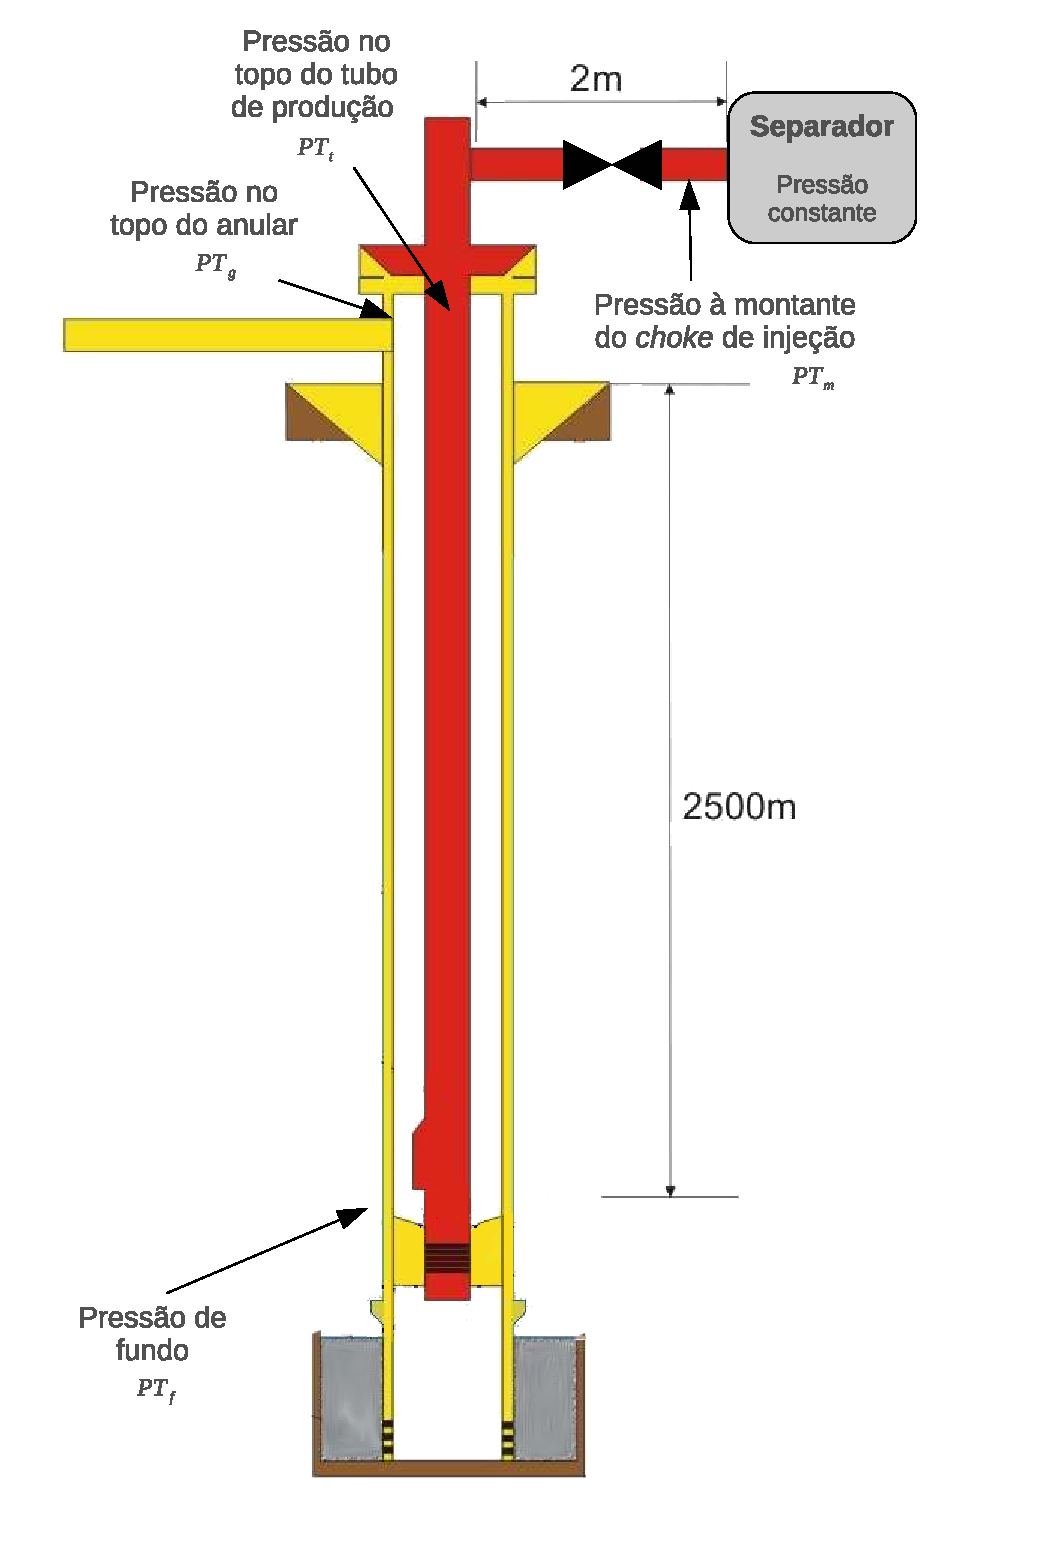
\includegraphics[height=.8\textheight]{figures/poco.eps}
%         \end{figure}
%         \column{.55\textwidth}
%         \begin{itemize}
%             \item 4 simulated pressure sensors:\vspace{-.5cm}
%                 \begin{itemize}
%                     \item bottom hole (PT$_f$)
%                     \item top of the production pipe (PT$_t$)
%                     \item top of the annular space (PT$_g$)
%                     \item upstream of the injection choke (PT$_m$)
%                 \end{itemize}
%             \item Data collected during 225 hours of well production
%             \item Sample rate of 1 sample per minute
%             \item White noise of NSR (noise to signal ratio) equal to $0.3$
%             \item The first 90 hours of data were used to develop the model
%         \end{itemize}
%     \end{columns}
% \end{frame}
% 
% \begin{frame}{Predictions for Simulated Data Set}
%     \vspace*{-.25cm}
%     \begin{figure}[!htb]
%         \centering
%         \includegraphics[width=\textwidth]{figures/pred_124d.eps}
%     \end{figure}
% \end{frame}
% 
% \begin{frame}{Sensibility Analisys for Simulated Data}
%     \begin{table}[!bt]
%         \centering
%         \begin{tabular}{lcc}
%             & AAKR-KF-SPRT & AAKR-SPRT\\
%             \midrule
%             MSE & $9.1293\times 10^{-3}$ & $2.8491\times 10^{-3}$ \\
%             $\mbox{S}_A$ & $1.9431\times 10^{-5}$ & $5.0840\times 10^{-5}$ \\
%             $\mbox{S}_C$ & $8.1022\times 10^{-5}$ & $11.8895\times 10^{-5}$ \\
%             \bottomrule
%         \end{tabular}
%     \end{table}
%     \vspace{1cm}
%     Note: MSE is calculated for unfaulted data.
% \end{frame}
% 
% \begin{frame}{Residual Analisys Without KF}
%     \vspace*{-.2cm}
%     \begin{figure}[!htb]
%         \centering
%         \includegraphics[width=\textwidth]{figures/res_124d.eps}
%     \end{figure}
% \end{frame}
% 
% \begin{frame}{Residual Analisys With KF}
%     \vspace*{-.2cm}
%     \begin{figure}[!htb]
%         \centering
%         \includegraphics[width=\textwidth]{figures/kfres_124d.eps}
%     \end{figure}
% \end{frame}
% 
% \subsection{Real Data Set}
% 
% \begin{frame}{Real Data Set}
%     \begin{itemize}
%         \item Pressure data collected from 3 sensors:
%             \begin{itemize}
%                 \item PDG (at the bottom hole)
%                 \item TPT (at the christmas tree)
%                 \item at the upstream of the injection choke (PT$_m$)
%             \end{itemize}
%         \item Data collected during 955 hours
%         \item Sample rate of 1 sample per minute
%         \item The first 500 hours were used to develop the model
%     \end{itemize}
% \end{frame}
% 
% \begin{frame}{Predictions for Real Data Set}
%     \vspace*{-.2cm}
%     \begin{figure}[!htb]
%         \centering
%         \includegraphics[width=\textwidth]{figures/pred_real_23d.eps}
%     \end{figure}
%     %%
%     % Artificial linear drift was inserted
%     % Upstream of the injection choke
%     % Downhole pressure, wellhead pressure
% \end{frame}
% 
% \begin{frame}{Sensibility Analisys for Real Data Set}
%     \begin{table}[!bt]
%         \centering
%         \begin{tabular}{lcc}
%             & AAKR-KF-SPRT & AAKR-SPRT\\
%             \midrule
%             MSE & $2.7013$ & $1.4061$ \\
%             $\mbox{S}_A$ & $0.0747$ & $0.6956$ \\
%             $\mbox{S}_C$ & $0.0466$ & $0.1208$ \\
%             \bottomrule
%         \end{tabular}
%     \end{table}
% \end{frame}
% 
% \begin{frame}{Residual Analysis Without KF}
%     \vspace*{-.2cm}
%     \begin{figure}[!htb]
%         \centering
%         \includegraphics[width=\textwidth]{figures/akres_real.eps}
%     \end{figure}
% \end{frame}
% 
% \begin{frame}{Residual Analysis With KF}
%     \vspace*{-.2cm}
%     \begin{figure}[!htb]
%         \centering
%         \includegraphics[width=\textwidth]{figures/kfres_real.eps}
%     \end{figure}
% \end{frame}
% 
% \section{Conclusions}
% \subsection{}
% 
% \begin{frame}{Conclusions and Future Works}
%     \begin{itemize}
%         \item Sensors play important roles in the oil field
%         \item Two on-line calibration monitoring systems were presented
%         \item Data-driven approach
%         \item The KF allows much \alert{less sensitivity} for drifts with a slight loss of
%             accuracy
%         \item The systems allows a greater extension of the \alert{useful life} of the sensors
%         \item Future works:
%             \begin{itemize}
%                 \item Uncertainty analysis
%             %% instead of statistical algorithms for drift detection
%                 \item Detection of valve closing
%                     \begin{itemize}
%                         \item variables decoupling
%                     \end{itemize}
%                 \item Automatic variables grouping
%             %% Which could be choose optimal groups of variables
%             \end{itemize}
%     \end{itemize}
% \end{frame}


\end{document}
